\chapter{Introduction}

%%%%%%%%%%%%%%%%%%%%%%%%%%%%%%%%%%%%%%%%%%%%%%%%
\section{Motivation}

Ambisonics is a spatial audio theory based on the directional decomposition of the sound field. Conceived in its primal form during the 70s \cite{gerzon1973periphony}, it was not until the 21st century, with a modern mathematical formulation \cite{daniel2000representation} and much more computational power available, that it definitely drew the attention of the research community. 


%\begin{figure}[t]
%  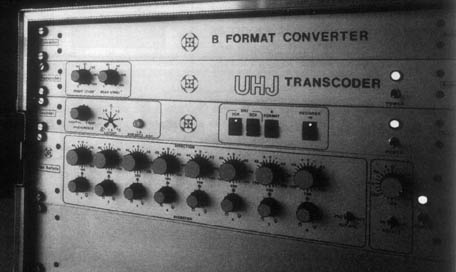
\includegraphics[width=\textwidth]{Figures/Introduction/hardware.jpg}
%    \caption{An ambisonic hardware processor, manufactured by Audio \& Design Recording Ltd. Source: \href{https://commons.wikimedia.org/w/index.php?curid=11813129}{Relen, Wikimedia Commons}}
%  \label{fig:hardware}
%\end{figure}

Nevertheless, the greatest contributor to the current interest in ambisonics has been the rise of Virtual Reality (VR) in recent years.
Although VR focuses primarily on visual cues, the immersive experience might be greatly enhanced by spatial audio \todo{CITE REQUIRED, begault?}. In this context, Ambisonics has been rapidly adopted as \textit{de facto} standard for spatial audio transmission, supposedly due to a variety of factors:

\begin{description}

  \item [Layout independence] As opposed to other audio spatialization techniques that rely on specific playback layouts, ambisonics makes use of an intermediate sound field representation, known as \textit{B-Format} (or just ambisonic audio). This representation, often referred to as \textit{scene-based}, can be then further processed to match any playback configuration. 

  \item [Recording device independence] Regardless of the specific characteristics of an ambisonic microphone, the recorded signal is usually converted into B-Format, which effectively represents the standard exchange format. 

  \item [Ease of manipulations] Signal-independent transformations of the ambisonic stream, and specifically rotations, are computationally inexpensive.

  \item [Binaural transformation] Spatial audio in VR is mostly consumed as binaural; methods for ambisonic to binaural conversion have been known for a long time \todo{cite?}. Furthermore, VR headsets can easily provide head rotation information, which can be used in combination with scene rotations to provide head-locked audio, which greatly improves immersiveness \todo{cite required!}. This is a key feature of ambisonics when compared to static binaural recordings.

\end{description}

Coming back to the Virtual Reality popularity, the following three events might be representative of the growth that it experienced in the second half of the 2010s: 
(i) the billionaire acquisition by Facebook of the VR headset manufacturer Oculus, in March 2014 \cite{facebookoculus}; 
(ii) the Time cover page devoted to VR: \textit{""The surprising joy of Virtual Reality. And why it's about to change the world"} (August 2015) \cite{time};
and (ii) M. Zuckerberg's invited talk at the \textit{Samsung Unpacked} event within the World Mobile Congress 2016 in Barcelona: \textit{"VR is the next platform where anyone can experience anything they want"} \cite{bbcnews}.


\begin{figure}[t!]
  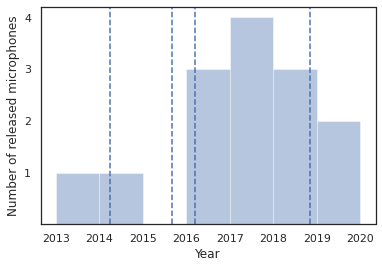
\includegraphics[width=\textwidth]{Figures/Introduction/num_mics_ticks.png}
  \caption{Number of ambisonic microphones released in last years (from \cite{List_of_Ambisonic_hardware}). From left to right, the vertical lines correspond to (i) Oculus acquisition, (ii) Time cover page on VR, (iii) M. Zuckerberg's speech in MWC, and (iv) Jaunt announcement of shift towards AR.}
  \label{fig:nummics}
\end{figure}


\begin{table}[t!]
\centering
\caption{List of ambisonic microphones released in recent years (from \cite{List_of_Ambisonic_hardware}).}
\begin{tabular}{cccc}
  \toprule
Manufacturer & Model   & Year & Order \\
\midrule
MH Acoustics & EigenMike   & 2013                     & 4                         \\
Brahma       & (Brahma)                                                   & 2014                     & 1                         \\
Sennheiser   & Ambeo                                                      & 2016                     & 1                         \\
Twirling     & 720 VR    & 2016                     & 1                         \\
Zoom         & H2n                                                        & 2016                     & 1                         \\
Zylia        & ZM-1                                                       & 2017                     & 3                         \\
Twirling     & 720 Lite    & 2017                     & 1                         \\
Ricoh        &  TA-1        & 2017                     & 1                         \\
Nevaton      & Nevaton VR                                                 & 2017                     & 1                         \\
Rode         &  Rode NT-SF1 & 2018                     & 1                         \\
CoreSound    &  OctoMic     & 2018                     & 2                         \\
Zoom         & H3-VR                                                      & 2018                     & 1                         \\
Brahma       & Brahma 8                                                   & 2019                     & 2                         \\
Voyage Audio & Spatial Mic  & 2019    & 2  \\
\bottomrule
\end{tabular}
\label{tab:nummics}
\end{table}


Given this context, many microphone manufacturers and audio-related companies have followed the industry trend in the search for new markets. Only in the interval 2016-2019, 12 different ambisonic microphones have reached the market (Figure~\ref{fig:nummics}) --- a greater amount than all previous existing ambisonic microphones together. A comprehensive list of recent ambisonic microphone releases is shown in \ref{tab:nummics}.


At the present time, however, the high expectations in VR have significantly lowered, as shown in Figure~\ref{fig:vrfunding}. This is due to a variety of reasons, including lack of interesting content and the high production cost of the headsets \cite{fortune}. The change of focus of Jaunt (formerly one of the biggest VR film production companies) towards Augmented Reality (AR), as of October 2018, might be a paradigmatic example of this tendency \cite{theverge}. 

\begin{figure}[t!]
  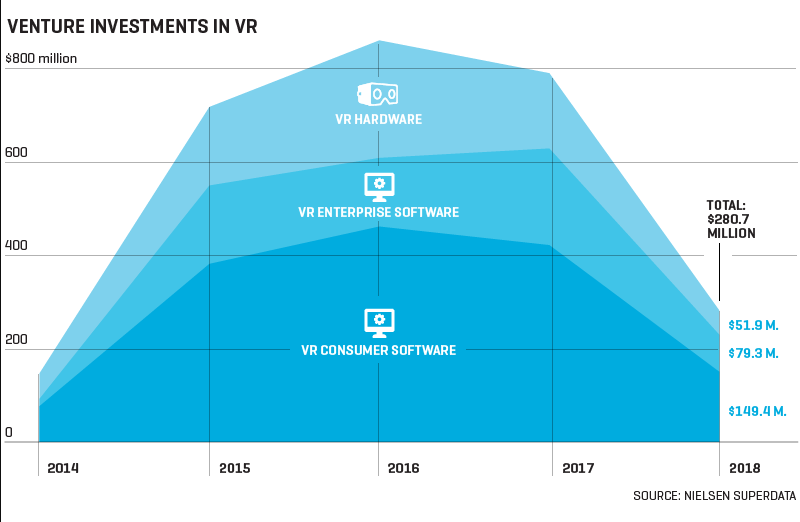
\includegraphics[width=\textwidth]{Figures/Introduction/vr_funding.png}
  \caption{Venture investments in VR in the period 2014-2018. Adapted from \cite{fortune}.}
  \label{fig:vrfunding}
\end{figure}



In any case, the current high availability and affordability of ambisonic microphones brings new challenges from the signal processing perspective. More specifically, ambisonic microphones conform a subset of near-coincident spherical microphone arrays, a category which possesses some specific characteristics.

Although the VR momentum has also reached spherical microphone array processing, many challenges remain still opened, and the number of research works specifically focusing on such geometry are still low. 
Besides that, the growing interest in AR posses new problems related to acoustical signal processing. But since ambisonics is still the standard choice for immersive audio, existing solutions might be successfully adapted. 

Lastly, the advance in signal processing methods for ambisonics can give rise to applications that enhance the work of immersive audio producers, providing meaningful information about the recorded scenes and automating some of the repetitive tasks, thus allowing a more flexible and creative workflow.










%%%%%%%%%%%%%%%%%%%%%%%%%%%%%%%%%%%%%%%%%%%%%%%%
\section{Problem Description}

\begin{figure}[hbt]
  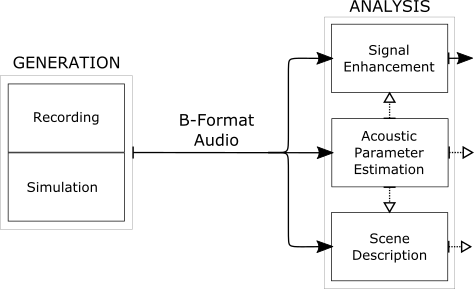
\includegraphics[width=\textwidth]{Figures/Introduction/SCHEME1.png}
  \caption{\todo{todo caption}}
  \label{fig:scheme1}
\end{figure}

EXPLAIN PARTS OF FIGURE:

Different levels of applications in multichannel acoustic signal processing (inspired by \cite{jarrett2017theory})

\begin{itemize}
	\item Acoustic Parameter Estimation (low level, audio2data)
	\begin{itemize}
		\item Direction of Arrival estimation
		\item Coherence analysis
		\item Acoustic description (RT60, etc)
		\item Source counting
	\end{itemize}

	\item Signal Enhancement  (high level, audio2audio)
	\begin{itemize}
		\item Source Separation
		\item Dereverberation / denoising
		\item IR estimation
	\end{itemize}

	\item Scene Description (high level, audio2data)
	\begin{itemize}
		\item Event Detection
		\item Acoustic Scene Classification
	\end{itemize}
\end{itemize}


%%%%%%%%%%%%%%%%%%%%%%%%%%%%%%%%%%%%%%%%%%%%%%%%
\section{Scientific Objectives}

preguntas cientificas concretas, coincidiendo con contribuciones

(base para la conclusion)

%\section{Goals}
%
%Research question: How can we exploit the characteristics of ambisonic recordings in order to extract signal-dependent, meaningful information from them? 


%%%%%%%%%%%%%%%%%%%%%%%%%%%%%%%%%%%%%%%%%%%%%%%%
\section{Outline}

\begin{figure}[t]
  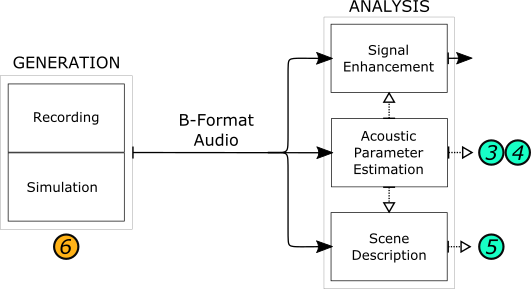
\includegraphics[width=\textwidth]{Figures/Introduction/SCHEME1_NUMBERS.png}
  \caption{\todo{todo caption}}
  \label{fig:scheme1_numbers}
\end{figure}

The present Thesis is organised as follows. 

\textbf{Chapter~\ref{chap:scientific}} introduces the basic concepts that will be developed throughout the Thesis, including spherical harmonics and ambisonics, coherence estimation, parametric analysis or room acoustics. The Chapter also defines the signal models and the mathematical terminology.


Chapters~\ref{chap:rt60}, \ref{chap:coherence} and \ref{chap:seld2019} develop the most significant academic contributions of the Thesis. 
\textbf{Chapter~\ref{chap:rt60}} presents a novel method for blind reverberation time in ambisonic recordings. To the best of our knowledge, this is the first method proposal specifically focusing on that problem.   The method is based on a Multichannel Auto-Regressive model of the late reverberation, which allows for an effective dereverberation of the ambisonic sound scene, and enables computation of the reverberation time from an estimation of the room impulse response. The evaluation metrics show a method performance similar to other state-of-the-art methods. 
\textbf{Chapter~\ref{chap:coherence}} analyses the response of tetrahedral microphone arrays, which are the simplest and most common form of ambisonic microphones, under spherically isotropic sound field. The analysis is performed using both simulated and recorded diffuse field, and the results quantify the differences between ideal and real values under a variety of conditions and estimators.  
In \textbf{Chapter~\ref{chap:seld2019}}, a complete system for Sound Event Localization and Detection of ambisonic sound scenes is described. The algorithm comprises two different parts. First, a parametric analysis is performed on the ambisonic signal. The analysis yields spatial localization and temporal activities of the sound events present in the scene. Then, each of those events is assigned to a class label by means of a deep-learning classifier. The method is able to perform in a similar way to the baseline system, while greatly improving its localization capabilities.

Finally, \textbf{Chapter~\ref{chap:data}} presents some libraries and software utilities developed throughout the Thesis. All the code has been publicly released under open source licenses. The libraries include utilities for the creation of datasets, the storage and exchange of impulse response files in a standard way, and the implementation of convenience tools for acoustic and microphone array signal processing analysis. Although the libraries do not directly involve any scientific contribution, they can be a great help for scientific and innovative purposes; given the industial nature of the candidate's doctoral program, we have considered relevant to include them in the present Thesis. \todo{check}

In order to place the different chapters within the problem context described in Section~\ref{sec:context}, we add to Figure~\ref{fig:scheme1} the Chapter numbers with our contributions, obtaining Figure~\ref{fig:scheme1_numbers}.




\section{Context}
\label{sec:context}



%%%%%%%%%%%%%%%%%%%%%%%%%%%%%%%%%%%%%%%%%%%%%%%%
\section{Contributions}


In the following list we show the main scientific contributions of the Thesis, organised by Chapters:

\begin{itemize}

	\item Chapter 3:\\
	\textbf{"Blind reverberation time estimation from ambisonic recordings"}.
	\underline{A. P\'erez-L\'opez}, A. Politis and E. G\'omez.
	Submitted to \textit{IEEE 22nd International Workshop on Multimedia Signal Processing, 2020.}
	
	\item Chapter 4:\\
	\textbf{"Analysis of spherical isotropic noise fields with an A-Format tetrahedral microphone"}.
	\underline{A. P\'erez-L\'opez} and N. Stefanakis.
	\textit{The Journal of the Acoustical Society of America 146.4 (2019): EL329-EL334.}

	\item Chapter 5:\\
	\textbf{A hybrid parametric-deep learning approach for sound event localization and detection.}
	\underline{A. P\'erez-L\'opez}, E. Fonseca and X. Serra.
	In \textit{Proceedings of the Detection and Classification of Acoustic Scenes and Events 2019 Workshop (DCASE2019)}.
	
	\todo{DCASE2020}
	
	\item Chapter 6:\\
	\textbf{Ambiscaper: A Tool for Automatic Generation and Annotation of Reverberant Ambisonics Sound Scenes}.\\
	\underline{A. P\'erez-L\'opez}.
	In \textit{16th International Workshop on Acoustic Signal Enhancement (IWAENC). IEEE, 2018.}
	
	\textbf{Ambisonics directional room impulse response as a new convention of the spatially oriented format for acoustics.}
	\underline{A. P\'erez-L\'opez} and J. De Muynke.
	In \textit{Audio Engineering Society Convention 144. Audio Engineering Society, 2018.}
	
	\textbf{pysofaconventions, a Python API for SOFA.}
	\underline{A. P\'erez-L\'opez}.
	In \textit{Audio Engineering Society Convention 148. Audio Engineering Society, 2020.}
	
	\textbf{A Python library for Multichannel Acoustic Signal Processing.}
	\underline{A. P\'erez-L\'opez} and A. Politis.
	In \textit{Audio Engineering Society Convention 148. Audio Engineering Society, 2020.}
	
\end{itemize}


Moreover, as a result of the development of the Thesis, the following open-source libraries have been implemented and released. All of them are available through the author's GitHub page, \url{https://github.com/andresperezlopez}: \todo{describir cada uno? con respecto a paper o chapter?}

\begin{itemize}

	\item rt60 estimation: \todo{todo}
	
	\item \href{https://github.com/andresperezlopez/DCASE2019_task3}{DCASE2019\_task3}

	\item \href{https://github.com/andresperezlopez/ambiscaper}{ambiscaper} 
	
	\item \href{https://github.com/andresperezlopez/pysofaconventions}{pysofaconventions}
	
	\item \href{https://github.com/andresperezlopez/masp}{masp: Multichannel Acoustic Signal Processing library}
	
\end{itemize}



